\setchapterpreamble[u]{\margintoc}
\chapter{Introduction} 
\labch{intro}

% Importance of multiphase interfacial flows 
\begin{marginfigure}
\centering
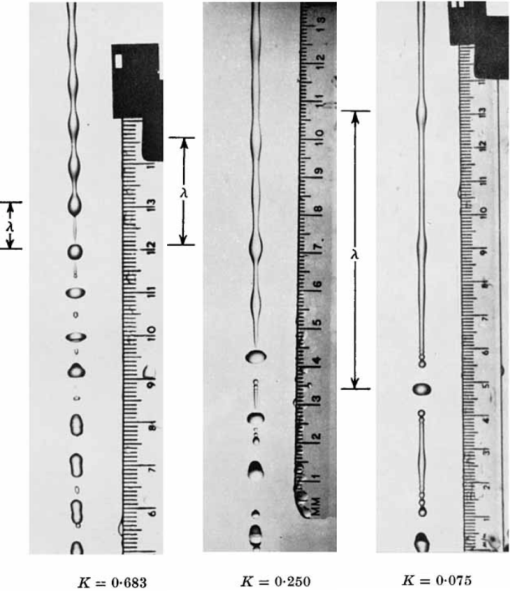
\includegraphics{plots/intro/jet.pdf}
\caption{Decay of a liquid jet into droplets driven by the growth of capillary instabilities corresponding 
	to different excitation frequencies. Image reproduced from Rutland and Jameson \cite{rutland1971non}.
	} 
\label{jet}
\end{marginfigure}

The dynamics of liquid-gas interfacial flows play a critical role in several processes in nature, 
as well as in myriad industrial applications. 
The key elements of surface tension dominated flows such as droplets and bubbles constitute the  
fundamental mechanisms governing the exchange of heat and mass at the ocean-atmosphere interface \cite{seinfeld1998air,deike}, 
mixing/separation in context of metallurgical processes \cite{johansen1988fluid,metal},  
conventional modes of heat transfer \cite{deckwer1980mechanism,bubble}
and ever so importantly, the tranmission of pathogens \cite{lydia_1,lydia_2}. 
One of the most fascinating features of multiphase flows is the process of atomization, 
in which a liquid volume transitions into smaller fragments via a series of topological 
changes of varying complexity, ultimately resulting in the emergence of drops of various sizes
driven by the action of capillary forces at the interface separating the fluids.  
Such processes are ubiquitous in a diverse range of applications spanning from combustion related processes 
(\cite{lefebvre2017atomization,bayvel1993liquid}) to agricultural irrigation (\cite{lake1977effect,reichenberger2007mitigation}).    

% Decay of jets, shear induced atomization, expansion of sheets , hole expansion in sheets, secondary atomization of drops 
Although liquid atomization is basically the transformation of a compact volume into drops,
this simplistic view masks the intricate interplay between inertia, viscosity and capillarity across 
different length and time scales spanning several orders of magnitude.  
Such non-trivial interactions are responsible for the abundant variety in the sequence 
of toplogical progressions that eventually lead to the formation of stable drops. 
The most basic transition involves the breakup of a cylindrical filament structure 
(see Fig. \ref{jet}) at approximately regular intervals, driven primarily by the 
growth of long wavelength perturbations due to capillary forces. 
A slightly more complicated transition involves liquid sheets (refer to Fig. \ref{spread}), 
where the inertial expansion of the sheet is opposed by the capillary deceleration of the edges,
resulting in the formation of liquid rims due to volume accumulation at the edges, 
the subsequent destabilization of which leads to the generation of drops. 
Sticking to the breakup of liquid sheets, another imporant transition involves the  
appearance of perforations or holes (see Fig. \ref{holes}) when the thickness of the sheet reaches a certain limit. 
The ensuing rapid expansion of such perforations due to capillary retraction results in the formation of drops. 
Arguably, the most convoluted route to drop formation in encountered when macroscopic 
liquid structures are subjected to shear-driven instabilities (see Fig. \ref{shear}) that 
arise at the interface due to the differential gas and liquid velocities. 
These primary instabilities of the Kelvin-Helmholtz \cite{khi} variety lead to the creation 
of a plethora of secondary structures, many of them corresponding to the aforementioned 
topologies like filaments, expanding sheets with rims, expanding holes in thin sheets etc 
amongst numerous others. The evolution and concomitant disintegration of such a diverse range
of structures lead to the production of drops with ample dispersion in their sizes.  
In view of the broad spectrum of liquid fragmentation phenomena that pique our scientific interest, 
the present body of work is be divided across two central themes :  

\begin{itemize}
	\item Development of numerical methods that can reproduce the dynamics of liquid-gas interfacial flows
		at low to moderate computational cost (spatial resolution), aimed towards flow configurations 
		involving significant contrasts in material properties across the interface. 
	\item Application of numerical methods in an effort to quantify the influence of certain topological
		characteristics of liquid structures on the resulting drop size distributions.  
\end{itemize}

\begin{marginfigure}
\centering
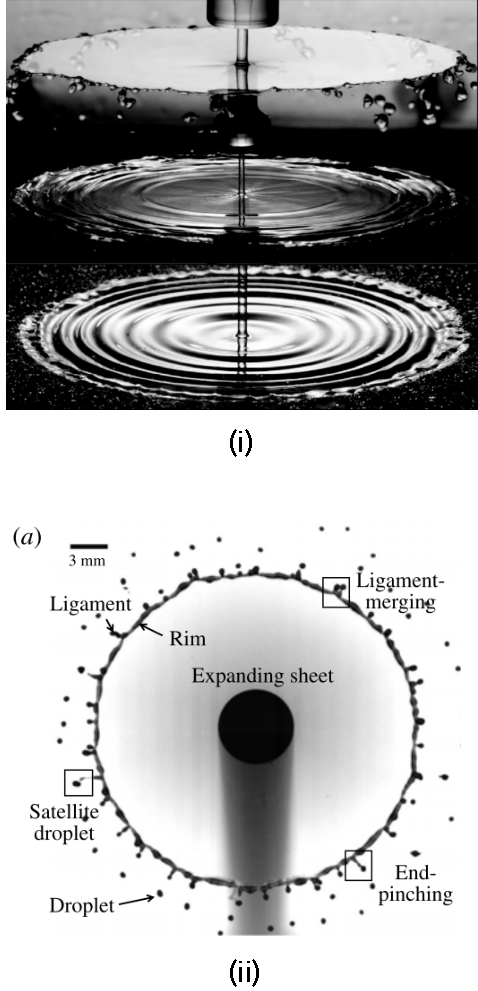
\includegraphics{plots/intro/spread.pdf}
	\caption{ Examples of steady and unsteady liquid fragmentation, demonstrating the disintegration of the  
	radially expanding liquid sheets driven by the capillary deceleration of the rims forming the edges of the sheet. 
	(i) Steady fragmentation of radially expanding sheets driven by jet impact, image reproduced from Bremond et al. \cite{bremond}.
	(ii) Unsteady fragmentation of liquid sheets following drop impact, image reproduced from Wang and Bourouiba \cite{lydia_3}.  
	}
\label{spread}
\end{marginfigure}

\Blindtext

\begin{marginfigure}
\centering
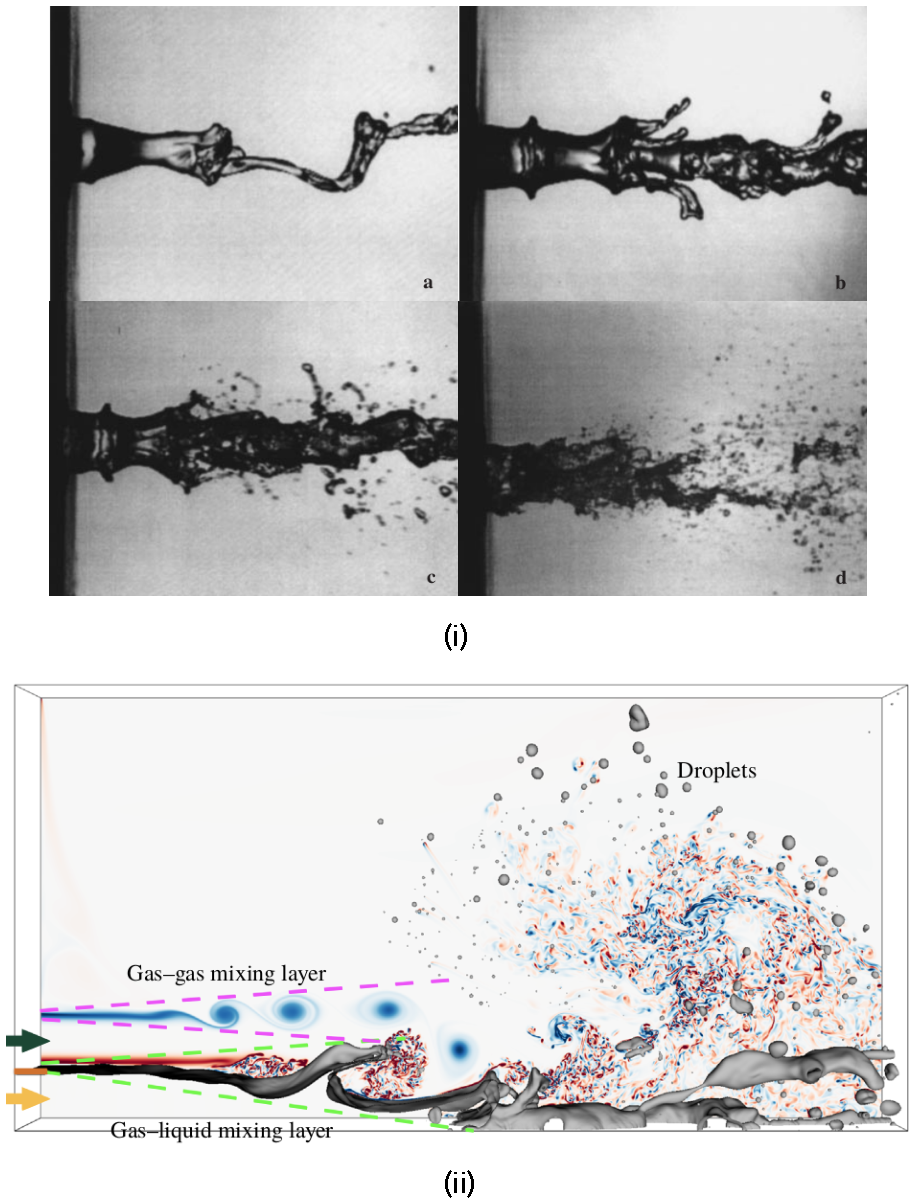
\includegraphics{plots/intro/shear.pdf}
	\caption{ Experimental and numerical investigations of liquid atomization 
	in which the primary stages of topological change are driven by shear instabilities. 
	(i) Liquid jet disintegration by a high speed coaxial gas flow, image reproduced from Lasheras and Hopfinger \cite{lasheras}.
	(ii) Atomization of a two-phase mixing layer between parallel liquid and gas streams, image 
	reproduced from Ling et al. \cite{ling}.
	}
\label{shear}
\end{marginfigure}

\blindtext

\begin{marginfigure}
\centering
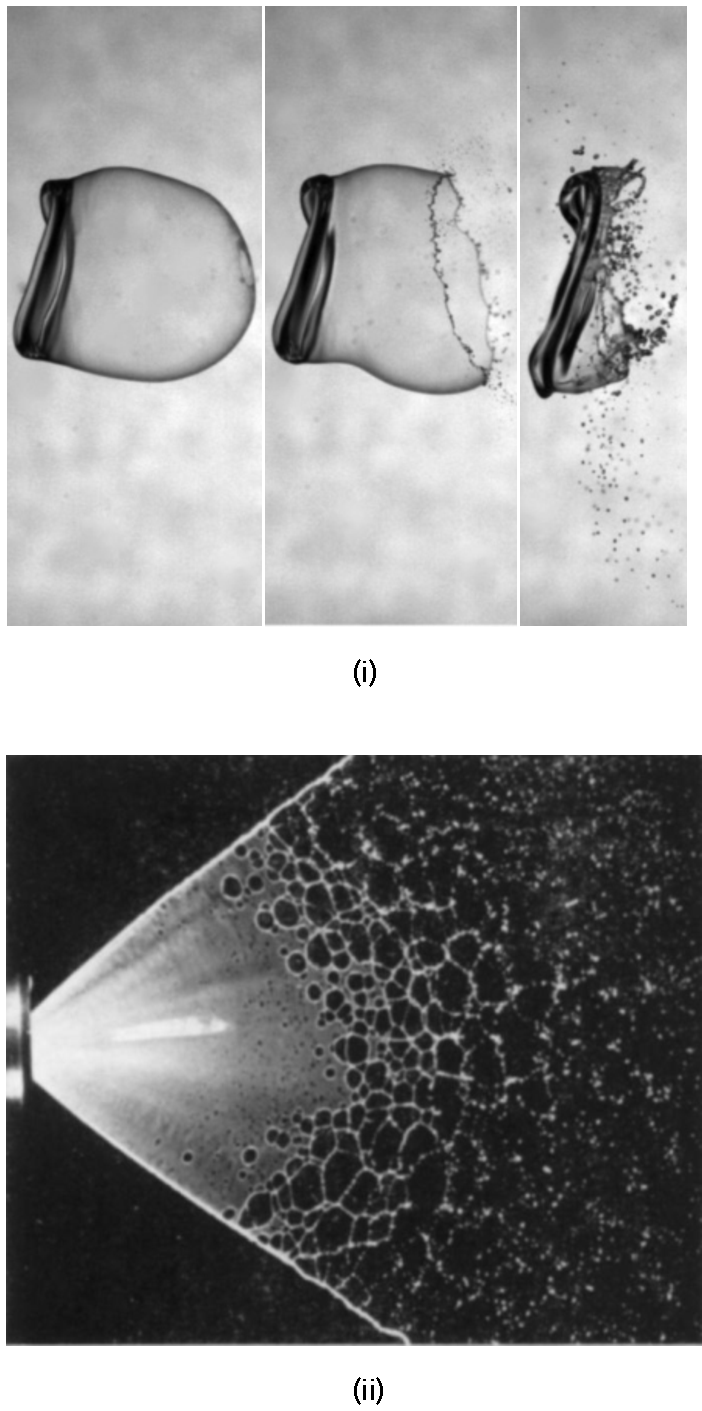
\includegraphics{plots/intro/holes.pdf}
\caption{ Liquid fragmentation triggered by the growth of perforations in thin liquid sheets. 
	(i) Secondary atomization (bag mode) of a drop in a crossflow, driven by the rapid capillary expansion of the hole. 
	Images reproduced from Opfer et al. \cite{hole_drop}.
	(ii) Effervescent atomization of expanding thin liquid sheets driven by the expansion of multiple perforations,
	image reproduced from Dombrowski and Fraser \cite{hole_sheet}.
	}
\label{holes}
\end{marginfigure}

\section*{Challenges in Numerical Modeling}

% Utility of numerical simulations, general info on interfacial tracking, Navier-Stokes 

% Artifical Atomization at low resolutions (raindrop crashes).

% Literature review of different attempts at momcons + summary tables

% Our Approach 


\section*{Polydispersity in Drop Sizes}

% Ligament mediated paradigm
% Breakup Regimes : Keller-Miksis inviscid, Paparouglou viscous, Eggers universal (inertio-visco) 

% Log-Normal, Gamma , Poisson distributions and underlying mechanisms

% Our approach


% Summary of parts and chapters in thesis
